\chapter{Implementation} \label{Implementation}

Pequeno rundown de como vamos a estar haciendo las varas.

For the creation of such a testing environment, four elements were recognized as of utmost importance to the validity of the tests and the author sought to implement them accordingly. In the following, they will be presented with detail, justifying the sources of the models and the parameter choices made.

The aforementioned elements are:

\begin{itemize}
	\item Generation and distribution of UEs
	\item Path loss (attenuation)
	\item Shadow Fading
	\item Random Access Procedure
\end{itemize}

\section{Generation and distribution of UEs} \label{PPP}
Often called a "completely" random proces, a Poisson process is a process where every event is stochastically independent of all other points in it, see \cite{Keeler2016}. This generation process is common in investigations about the performance of networks, as eloquently expressed by \cite{Keeler} In our case, the Poisson-distributed random variable are the number of points in the bounded region we are investigating. The distribution is described by the following probability mass function:

\begin{equation} \label{eq:Poisson}
P\left( x\ points\ in\ region \right) = \frac{{e^{ - \lambda } \lambda ^x }}{{x!}}
\end{equation}

By providing the $\lambda$ above, often called mean density (\cite{Keeler2016}), we can adjust the expected amount of points generated in a given area. In order to evaluate the robustness of different algorithms, the tests were made with a variety of $\lambda$ values. The generated amount of points are then distributed in the given area with a uniform distribution, where both the $x$ and $y$ value are distributed along the appropriate axis. In both cases, the \textit{Python} package \textit{NumPy} was utilized for the realization of the random distributions.

\begin{figure}[!h]
\centering
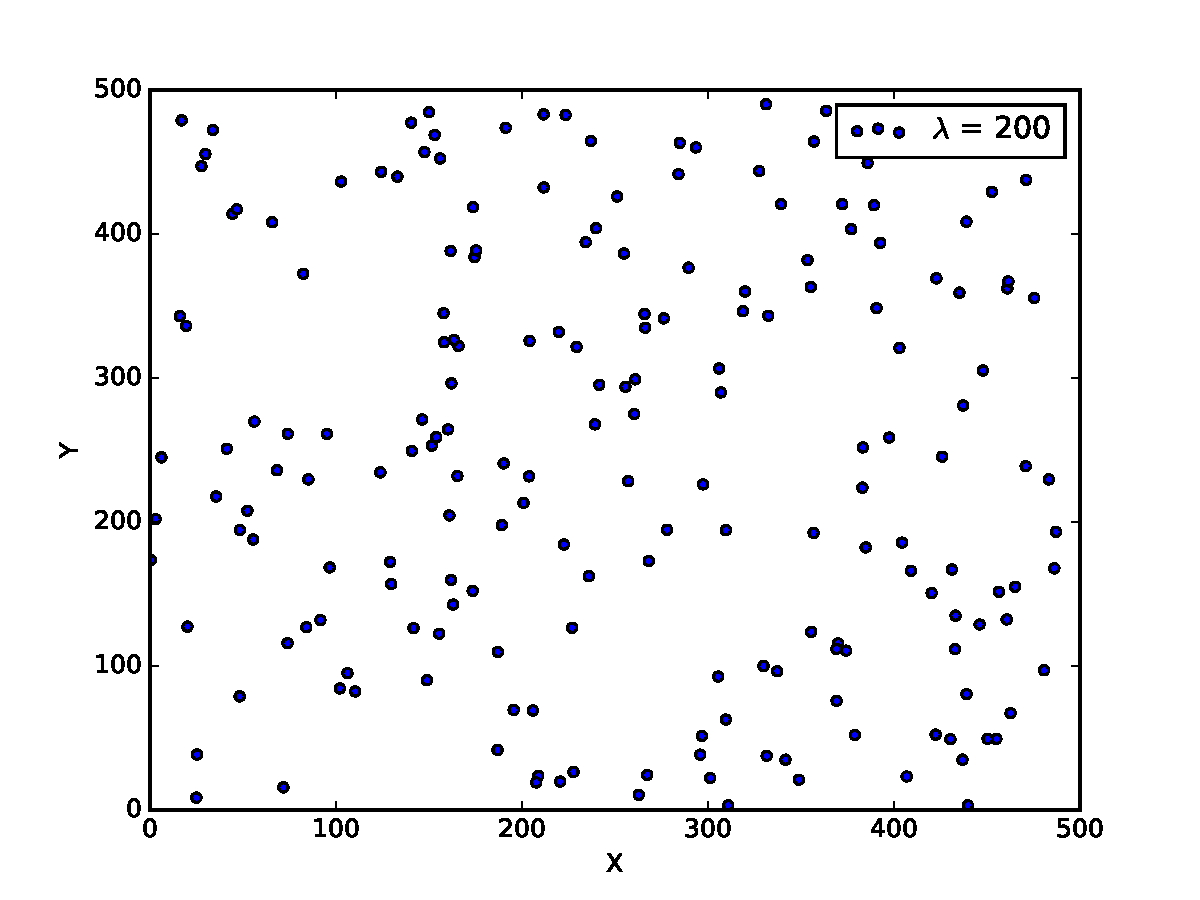
\includegraphics[scale = 0.6]{figures/PPP}
\caption{Example of a PPP with $\lambda = 200$}
\end{figure}

Thus we have generated the number and position of all our UEs according to a Poisson Point Process (PPP).

\section{Path loss (attenuation)} \label{PL}
Whenever transmission between devices is being investigated, loss due to attenuation as the signal propagates through space is an unavoidable topic. Distance degradates electromagnetic waves in terms of power in any real system and any simulation that does not reflect this phenomenon is simply not valid. 

In search of the best documented and most forward-looking models available, we settled on the use of METIS (Mobile and wireless communications Enablers for the Twenty-twenty Information Society), a EU Project that seeks to promote the definition of 5G mobile technologies. Its channel model, presented in its deliverables (\cite{Raschkowski}) was especially insightful. 

For the purposes of this thesis, the Stochastic Model, a "geometry-based stochastic channel model", was chosen for the way it lined up with our own goals, especially when it came to level of detail and complexity. Their figures are based on previous efforts by 3GPP studies to model these same phenomena. Due to the highly dense, urban system we are investigating, propagation scenatio number one, "Urban Micro" was selected. Due to the constraints of this thesis, we narrowed our focus on Outside-to-Outside (020) connections, although the integration of Outside-to-Inside (O2I) could be a feature of future research.

When calculating the attenuation for a given path between two devices, there emerge two distinct cases, depending on whether there are any significant obstacles between the two of them: Line-of-Sight (LOS) and Non-Line-of-Sight (NLOS).



\subsection{Manhattan Grid} \label{mh_grid}
In order to determine whether a given link is a LOS or NLOS link, we need information about the obstacles present in the path between the two. In our case, we don't consider objects like cars and people explicitly, but rather account for all such minor objects and reflections they might create with a stochastic model (see \ref{SF}). Buildings, on the other hand, represent such massive, nigh-impenetrable objects that we must contemplate them concretely.

The preferred method mentioned in the METIS deliverables is the use of a "Manhattan-like" grid, meaning a city-layout comprised of rectangular blocks criss-crossed by wide streets. To determine both the size and the overall layout of our Manhattan Grid, we again turn to the extensive work done by METIS. The measurements with which their relevant models were tested were run in Madrid, with a grid of around 500 meters of both length and width. We homogenized the scenario by having exclusively square blocks, but maintained both the street width and the general dimensions.


\begin{table}[htbp]
\begin{center}
 \begin{tabular}{||p{3cm}|p{3cm}||} 
 \hline
 \textbf{Parameter} & \textbf{Value}\\
 \hline\hline
 Grid Dimensions & 500 m $\times$ 500 m \\ 
 \hline
 Block Width & 110 m \\
 \hline
 Block Length & 110 m \\
 \hline
 Street Width & 20 m \\
 \hline
\end{tabular}
\end{center}
\caption{Video traces used for testing}
\end{table}

The introduction of an explicit grid raises the issue of the positioning of our UEs again. Having scattered them in a Poisson Point Process (see \ref{PPP}), some inevitably now find themselves inside a building and not on the street, as is necessary for our O2O simulations. We overcome this obstacle by simply finding the shortest route from the position inside a block to the street: as the UE position is random, so too is the route taken. Thus we avoid completely discarding the randomness of their positioning.

\begin{figure}
\centering
\begin{subfigure}{.35\textwidth}
  \centering
  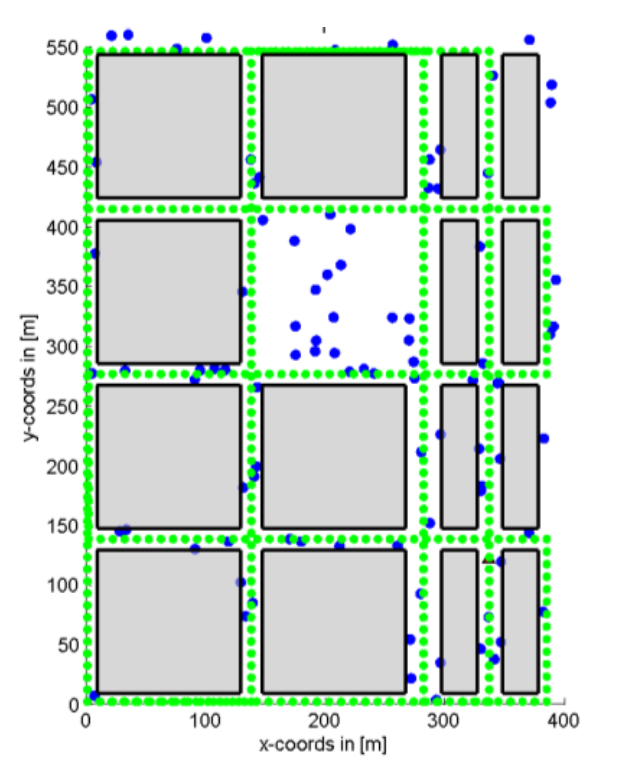
\includegraphics[width=1.2\linewidth]{figures/Madrid}
  \caption{Madrid grid \cite{Raschkowski}}
  \label{fig:sub1}
\end{subfigure}%
\begin{subfigure}{.65\textwidth}
  \centering
  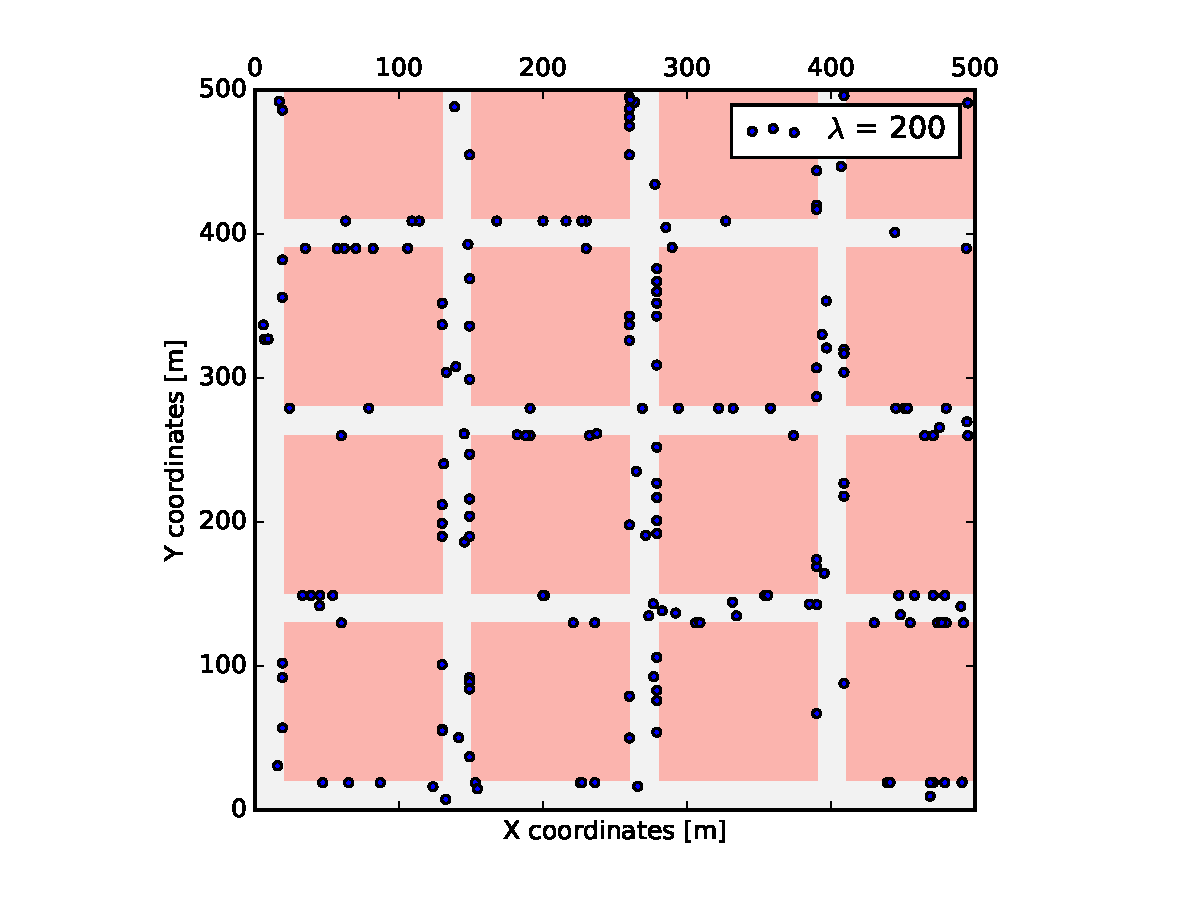
\includegraphics[width=1.058\linewidth]{figures/mh_grid}
  \caption{Own implementation, including moved UEs}
  \label{fig:sub2}
\end{subfigure}
\caption{Comparison between two Manhattan Grids}
\label{fig:test}
\end{figure}


With a Manhattan-like layout at the ready, questions about whether a link has LOS or not become much easier to answer.

\subsection{Line-of-Sight}
HOW DETAILED SHOULD I BE HERE ON THE FORMULAE?
If not at all maybe get rid of these subsections.

\subsection{Non-Line-of-Sight}
s.o.

\section{Shadow Fading} \label{SF}
As mentioned in \ref{mh_grid}, Shadow Fading - meaning the effects on the signal caused by smaller obstacles - as well as the reflections they create are modelled through a stochastic model. This type of fluctuation, called "Shadow Fading" or "long-term fading" is often realized through a Gaussian distribution in the logarithmic scale (also called a log-normal distribution), as asserted in \cite{Forkel2004} and shown below in its probability density function. In our case, we followed METIS specifications and set $\mu = 0$ and $\sigma_{L_s} = 7 dB$.

\begin{equation} \label{eq:SF}
p(L_s) = \frac{1}{{\sigma_{L_s} \sqrt {2\pi } }}e^{{{ - \left( {L_s - \mu_{L_s} } \right)^2 } \mathord{\left/ {\vphantom {{ - \left( {x - \mu } \right)^2 } {2\sigma_{L_s} ^2 }}} \right. \kern-\nulldelimiterspace} {2\sigma_{L_s} ^2 }}}
\end{equation}

While any given point is distributed randomly along the normal distribution, completely random and uncorrelated shadow fading variables make little sense when one considers that the effects of any given set of obstacles won't change much in the space of a couple of meters. In order to account for the necessary correlation that these shadow fading variables experience, a normalized autocorrelation function is introduced, both in \cite{Forkel2004} and \cite{Raschkowski}, with a decorrelation value suggested by METIS $d_{corr} = 8 m$.

\begin{equation} \label{eq:corr}
R(\Delta x) = e^{-\frac{|\Delta x|}{d_{corr}} ln(2)}
\end{equation}

After generating the shadow fading variables with equation \ref{eq:SF} and the autocorrelation coefficients with equation \ref{eq:corr}, both matrices are convoluted to generate the correlated values. Convolution does not alter the underlying distribution, but it does elicit a correction of the mean and standard deviation (compare with \cite{Forkel2004}) in order to return it to the values of the original Gaussian distribution. Our realization is shown below, both before and after the aforementioned correction for spatial correlation.